\documentclass{article}

\setlength{\parskip}{\baselineskip}
\setlength{\parindent}{0pt}
\usepackage[fontsize=12pt]{fontsize}
\usepackage{graphicx}
\usepackage[left=2cm,right=2cm,top=2cm,bottom=2cm]{geometry}
\usepackage{fancyhdr}
\usepackage{xcolor}
\usepackage{lastpage}
\usepackage{caption}
\usepackage{amsmath}
\usepackage{bm}
\pagestyle{fancy}
\renewcommand{\headrulewidth}{0pt}
\fancyhead{}
\cfoot{Page \thepage\ of \pageref{LastPage}}
\thispagestyle{fancy}
\setlength{\parindent}{0pt}


\begin{document}


\section*{\begin{center}
    Documentation of the Optional Interpolation Assessment
\end{center}}
\stepcounter{section}


\subsection{Summary}
The file ``ERT\rule{2mm}{0.15mm}interpolation.py'' contains the Python code
for interpolating the provided data onto a structured grid. 

\textbf{Requirements:} This code require the end user to have Python 3 install on 
their system. It is intended to be ran the the command prompt (see example below) 
or via an IDE such a Jupyter Notebooks.

Example usage in Windows command prompt:
\vspace{-5mm}
\begin{itemize}
    \item Run: ``python ERT\rule{2mm}{0.15mm}interpolation.py''
\end{itemize}

Example output:
\vspace{-5mm}
\begin{center}
    \fbox{ 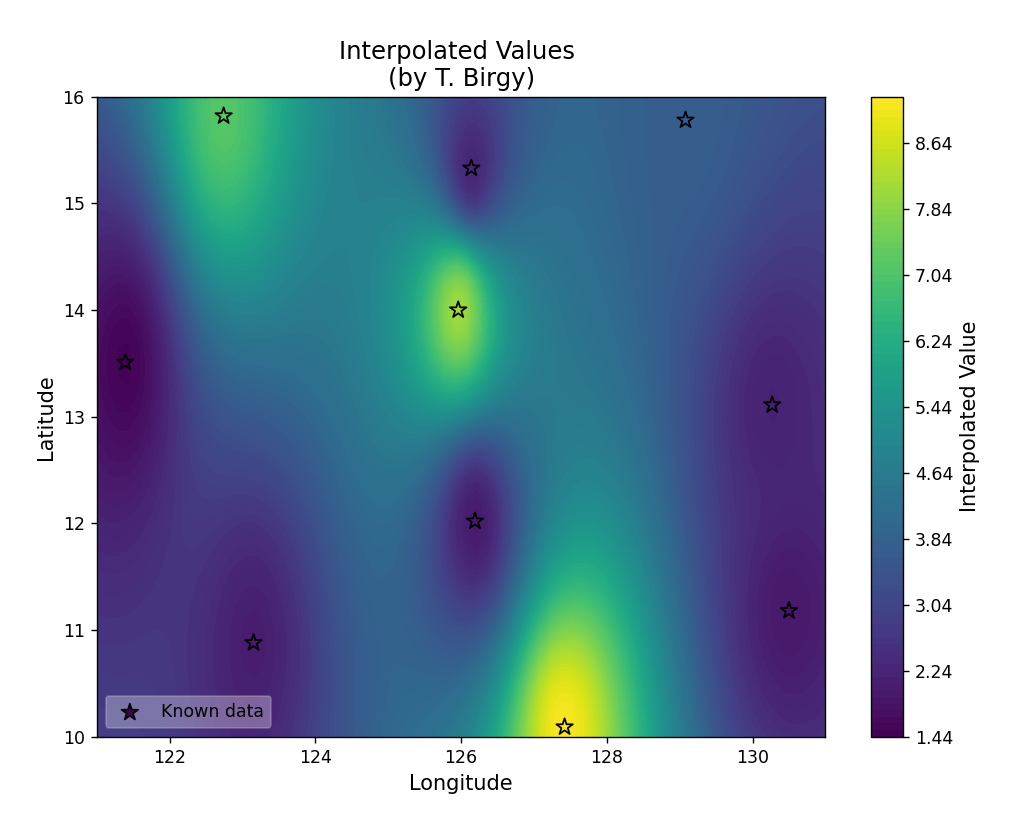
\includegraphics[width=0.75\textwidth]{interp_plot.PNG} }
\end{center}

\newpage
\stepcounter{section}
\subsection{Interpolation Methodology}
The provided data is given in Figure 1.
\begin{table}[h] 
    \centering
    \label{tab:example}
    \begin{tabular}{|c|c|c|} 
        \hline 
        \textbf{Longitude} 1 & \textbf{Latitude} 2 & \textbf{Value} \\ 
        \hline
        121.39 & 13.51 & 1.494 \\ 
        126.19 & 12.02 & 1.934 \\
        130.27 & 13.11 & 2.148 \\
        127.42 & 10.09 & 9.155 \\
        126.14 & 15.33 & 2.221 \\
        125.96 & 14.00 & 8.100 \\
        123.15 & 10.88 & 2.039 \\
        130.50 & 11.18 & 1.916 \\
        129.08 & 15.78 & 3.729 \\
        122.74 & 15.82 & 7.137 \\
        \hline
    \end{tabular}
    \caption{Table of provided data.}
\end{table}

\vspace{-5mm}
As this data does not exist on a regular grid, many typical interpolation methods 
(e.g., bilinear) are not appropriate. For this reason, inverse-distance weighting 
was used to compute the interpolation. This is a simple, yet flexible methodology 
which works well with irregularly spaced input data. 

This interpolation method assigns a value to a point $p$ based on the value of its 
neighboring points, with points closer to $p$ carrying more weight. Mathematically, 
points $p$ are calculated as follows.
\begin{equation}
    p(\bm{x}) = \begin{cases}
        \frac{ \sum_{i=1}^{N} p_i/ \left(d(\bm{x,x_i})\right)^r}{ \sum_{i=1}^{N} d(\bm{x,x_i})^{-r}} , & d(\bm{x,x_i}) \neq 0 \\
        p_i, & d(\bm{x,x_i}) = 0
    \end{cases}
\end{equation}

where $p(\bm{x}$ is the grid point being assigned an interpolation value, $N$ is the 
number of points from which to interpolate, $d(\bm{x,x_i})$ is the distance between 
the current grid point and the $i^\text{th}$ known point, and $r$ is the rate of 
decay. In addition, there are two important details which must be carefully considered. 

Firstly, since the grid values represent latitude and longitude over a large section 
of the Earth, a simple Cartesian distance is not appropriate as this would not 
properly account for curvature. Instead, the Haversine formula is used to calculate 
the magnitude of the range between the two points. 

Secondly, the lower summation of Eq. (1) is known to diverge when $r < D$, where $D$ 
is the dimension of the data. Since the provided data is 2D, a value of $r>2$ should 
be used. The current implementation uses a value of 2.1.







\end{document}